\chapter{Continuous Models}
Many engineered systems consist of computers, communications networks, and other digital (i.e., discrete event) systems whose purpose is to monitor and control a physical (electrical, mechanical, thermodynamic, etc.) process. Models of these systems have parts modeled as discrete event systems, parts modeled with continuous (differntial or differential-algebraic) equations, and the interaction of these parts is crucial to understanding the system's behavior. Where the continuous models interact with the discrete event models, these interactions are necessarily discrete. For example, a digital thermometer reports temperature in discrete increments, electrical switches are either open or closed, a threshold sensor is either tripped or it is not. Discrete interactions in a combined continuous-discrete event simulation are managed just as before; the models interact by producing output events and reacting to input events.

If, on the other hand, two systems interact continuously, then those interacting parts at least are modeled with continuous equations. In this case, accurate simulation is greatly facilitated by lumping the two systems into a single assembly; in \adevs\ this assembly is an \classname{Atomic} model that encapsulates the system's continuous dynamics. The essence of the approach to combined simulation in \adevs\ consists therefore of building atomic models that i) approximate the behavior of the continuous systems and ii) generates and consumes events at those instants when the continuous system interacts with a discrete event one.

There are three possibly outcomes of this lumping process. One possibility is that we end up with a single assembly; in this case our model is essentially continuous and we are probably better off using a simulation tool for continuous systems. At the other extreme, we find that the continuous parts of our model are very simple, yielding to analytical solutions that are easily transformed into discrete event models. Between these two extremes are models with continuous dynamics that are not simple but also do not dominate the modeling problem. The continuous system simulation part of \adevs\ is aimed at this type of model.

\section{Differential equation modeling with the \classname{ode\_system} class}
Models described by ordinary differential equations are implemented by subclassing the \classname{ode\_system} class. This class has two sets of methods: the first is for the model's continuous dynamics and the second is for the model's discrete event dynamics. I'll illustrate both with the simple, if somewhat contrived, example of a cherry bomb\footnote{A cherry bomb is a small red firecracker. They are dangerous, and illegal in the United States. Nonetheless, every school seems to have at least one obnoxious kid who likes to put them into toilets.}. This bomb is dropped from a height of 1 meter and bounces until it either explodes or is doused with water. We'll assume that the cherry bomb only bounces up and down and is perfectly elastic. The cherry bomb explodes 2 seconds from the time it is lit and dropped unless doused first. Dousing the cherry bomb puts out the fuse\footnote{Cherry bomb fuses are frequently water proofed.}. Dousing is a discrete input event and the cherry bomb produces a discrete output event if it explodes. 

This model has two continuous state variables: the height and velocity of the cherry bomb. Between events, these variables are governed by the pair of differential equations
\begin{align}
&\dot{v} = -9.8 \label{eqn:v} \\
&\dot{h} = v \label{eqn:h}
\end{align}
where $9.8$ meters per second per second is acceleration due to gravity, $v$ is velocity, and $h$ is height. In this example, it is also useful to know the current time. We keep track of this by adding one more differential equation
\begin{equation}
\dot{t} = 1 \label{eqn:t}
\end{equation}
whose solution is $t_0 + t$ or just $t$ if we set $t_0 = 0$. The ball bounces when it hits the floor, and bouncing causes the ball's velocity to change sign; specifically
\begin{equation}
h = 0 \ \& \ v < 0 \implies v \leftarrow -v \label{eqn:state_event}
\end{equation}
where $\implies$ is logical implication and $\leftarrow$ indicates an assignment. 

Equations \ref{eqn:v}, \ref{eqn:h}, and \ref{eqn:t} are the state variable derivatives, and these equations are implemented in the \methodname{der\_func} method of the \classname{ode\_system} class. The signature for this method is
\begin{verbatim}
void der_func(const double* q, double* dq)
\end{verbatim}
The q pointer is the array of state variable values; in this case $h$, $v$, and $t$. The dq pointer is the array of state variable derivatives; in this case $\dot{h}$, $\dot{v}$, and $\dot{t}$. When the simulator calls the der\_func method, it supplies q. In response, the method computes the values of $\dot{h}$, $\dot{q}$, and $\dot{t}$ and stores them in the dq array.

Equation \ref{eqn:state_event} is a state event condition and it is implemented in two parts. The \methodname{state\_event\_func} method implements the `if' part (left hand side) of the condition. The signature of this method is
\begin{verbatim}
void state_event_func(const double *q, double *z)
\end{verbatim}
Again, the supplied q array contains the current state variable values. These are used to evaluate the state event condition and store the result in the z array. The simulator detects state events by looking for changes in the sign of the z array entries. Note that the event condition should be continuous in the state variables on which it depends. In the case of the cherry bomb this is simple to do: we simply use $z=h$ if $v < 0$ and $z=1$ if $v >= 0$.  

The `then' part (right hand side) is implemented with the \methodname{internal\_event} method, which the simulator invokes when the state event condition is true. The signature of this method is
\begin{verbatim}
void internal_event(double *q, const bool *state_event)
\end{verbatim}
where, again, $q$ is the value of the state variables at the event. The entries of the array state\_event are true for each z in the state event condition array that evaluates to zero. This array therefore has one entry for each state event condition, and it has one additional entry to indicate time events, which are described below.

The cherry bomb has one discrete state variable with three possible values: the fuse is lit, the fuse is not lit, and the bomb is exploded. This variable changes in response to two events. The first event is when the bomb explodes; this is a time event that we know will occur 2 seconds from the time that the fuse it lit. The \methodname{time\_event\_func} method is used to schedule the explosion by returning the time remaining until the fuse burns out. The signature of the of this method is
\begin{verbatim}
double time_event_func(const double* q)
\end{verbatim}
As before, q is the current value of the state variables. The \methodname{time\_event\_func} is similar to the familiar \methodname{ta} method; it is used to schedule autonomous events based on the current value of the model's state variables. When this time expires, the simulator calls the \methodname{internal\_event} method with the last flag in the state event array set to true.

The second event that can change the state of the fuse is dousing with water. This an external event. External events, of course, are not scheduled by the model itself; they occur when and if the input event arrives. The \methodname{external\_event} method implements the response of the cherry bomb to dousing with water. Its signature is
\begin{verbatim}
void external_event(double *q, double e, const Bag<X> &xb)
\end{verbatim}
The array q contains the values of the continuous state variables, e is the time since the last discrete event, and xb is the bag of input. The douse event is an input and it appears in the input bag xb if the event occurs. 

As before, it is possible for an external and internal event to coincide. When this happens, the simulator calls the method \methodname{confluent\_event}. Its signature is
\begin{verbatim}
void confluent_event (double *q, const bool *state_event, const Bag<X> &xb)
\end{verbatim}
and its arguments are as described for the internal and external methods.

The cherry bomb model produces an output event when it explodes, and the \methodname{output\_func} method is use for this purpose. Its signature is
\begin{verbatim}
void output_func(const double *q, const bool *state_event, Bag<X> &yb)
\end{verbatim}
Its q and state\_event arguments are as described for the internal\_event method, and the bag yb is to be filled with the model's output. As with an \classname{Atomic} model, the output\_func is always invoked immediately prior to the internal\_event and confluent\_event methods.

All that remains in the implementation is to supply a \methodname{gc\_output} for collecting garbage, a constructor, and a method for initializing the continuous state variables. The gc\_output method works identically to that of the \classname{Atomic} class and so needs no more discussion here. The constructor for the cherry bomb must call the constructor of its \classname{ode\_system} base class. The signature of this method is
\begin{verbatim}
ode_system (int N_vars, int M_event_funcs)
\end{verbatim}
where N\_vars is the number of entries in the q and dq arrays (i.e., the number of continuous state variables) and M\_event\_funcs is the number of entries in the z and state\_event arrays (plus one for the time event). For the cherry bomb, N\_vars is three and M\_event\_funcs is one.

The constructor does not initialize the continuous state variables. Instead, the simulator calls the init method whose signature is
\begin{verbatim}
void init(double* q)
\end{verbatim}
and where q is an array that should be filled with the initial values for, in the case of the cherry bomb, $h$, $v$, and $t$. The complete implementation of the \classname{CherryBomb} is listed below.

Figure \ref{fig:cherry_bomb_trajectory} shows the cherry bomb trajectory from $t=0$ to its explosion at $t=2$. This plot was produced using the simulation program listed above. There is nothing particular surprising about it, but you can observe the discrete changes in the cherry bomb's trajectory. There are two bounce events at $t \approx 0.45$ and $t \approx 1.4$. The cherry bomb explodes abruptly at the start of its third decent.
\begin{figure}[ht]
\centering
\epsfig{file=cont_models_figs/ball_height.eps}
\caption{A simulation of the cherry bomb model that terminates when the cherry bomb explodes.}
\label{fig:cherry_bomb_trajectory}
\end{figure}
\section{Using the Runge-Kutte Integration Modules}
\adevs\ has two pre-built \classname{Atomic} models that can be used to simulation continuous systems. These two models are essentially the same; one uses a fixed step size, fourth order Runge-Kutte integration scheme to solve a set of ordinary differential equations and the other uses a variable step size, fourth/fifth order Runge-Kutte scheme to do the same thing. In general, you will probably prefer to use the variable step size scheme because it, unlike the fixed step size scheme, has a built in error control mechanism. Both models are used in exactly the same way, differing only in the parameters that are passed to their constructors.

The \adevs\ RK models are abstract classes with seven abstract methods that must be implemented by your derived class. The RK models are derived from the \classname{Atomic} class, but you will not be implementing the five familiar methods \methodname{delta\_int}, \methodname{delta\_ext}, \methodname{delta\_conf}, \methodname{ta}, and \methodname{output\_func}. But you will implement the familiar \methodname{gc\_output} method. It performs the same function in this new context, differing only in that it operates on objects produced by the new \methodname{discrete\_output} method. The remaining six new methods are used to describe the continuous dynamics of your model, to describe how your model generates and responds to discrete events, and to record the model's continuous trajectory. The methods are
\begin{verbatim}
void der_func(const double* q, double* dq)
void state_event_func(const double* q, double* z)
double time_event_func(const double* q)
void discrete_action(double* q, const Bag<X>& xb)
void discrete_output(const double* q, Bag<X>& yb)
void state_changed(const double* q)
\end{verbatim}
which are used, as the names suggest, to implement the state variable derivative functions and state event conditions, to schedule time events, to implement discrete state changes, to generate discrete outputs, and to take an action (usually recording the state trajectory in a file) when the integration scheme changes a state variable. 



\section{Building Numerical Integration Blocks for \adevs}
The \classname{rk45} and \classname{rk4} classes are not directly derived from the \classname{Atomic} class; they are actually derived from the \classname{DESS} class, which is derived from the \classname{Atomic} class. The \classname{DESS} (Differential Equation System Specification) class\footnote{The classification of dynamic systems into discrete event, discrete time, and continuous models is formalized by Zeigler in his book ``Theory of Modeling and Simulation". The acronyms for each class are DEVS (Discrete EVent system Specification), DTSS (Discrete Time System Specification), and DESS (Differential Equation System Specification).} replaces the five familiar \classname{Atomic} model methods with five new methods: 
\begin{verbatim}
virtual void discrete_output_func(Bag<X>& yb)
virtual void discrete_action_func(const Bag<X>& xb)
virtual void evolve_func(double h)
virtual double next_event_func(bool& is_event)
virtual void state_changed()
\end{verbatim}
Only the \classname{Atomic} model's \methodname{gc\_output} method is retained for the purposes of cleaning up objects created by the \methodname{discrete\_output\_func} method. The \classname{rk4} and \classname{rk45} classes were built by specializing these five methods; you can add new continuous system simulation algorithms to \adevs\ in the same way.

The method names are indicative of their function. The \methodname{state\_changed} method is used to notify the derived class when a new state is computed. The method is intended as a tool for saving state trajectories as a simulation progresses, and as such it is not really essential for modeling. The \methodname{state\_changed} method is invoked once at time zero (so that you can record the initial state), after every integration step, and before and after every discrete action (i.e., discrete state changes due to state, time, and input events).

The \methodname{next\_event\_func} method takes the place of the \classname{Atomic} class's \methodname{ta} method. The \methodname{next\_event\_func} returns the smallest of the next integration step size and the time remaining until next internal event time. The integrations step size is selected by the derived class; it could be a fixed value or chosen dynamically to satisfy error or stability constraints. The next internal event time is also selected by the derived class; it can be the known discrete event time (i.e., at time event) or the time of the next state event. The is\_event flag is an output argument; its value must be true if the next event is a time or state event and false if it is just an integration step. 

The \methodname{evolve\_func} is responsible for advancing the model's continuous trajectories. The method's role is to integrate the differential or differential algebraic equations that describe the model's continuous motion. The argument h is the step size that must be used; h is always less than or equal to the value given by the \methodname{next\_event\_func}. It is important to distinguish between the trial evaluations that might be required to pick the next integration step size and actually advancing the continuous trajectories. Many trial integration steps might be needed to implement the \methodname{next\_event\_func}; these trial steps might use different steps sizes to find one the gives a tolerable error or to locate state events in the continuous solutions. But when an appropriate time step has been found and given to the simulator via the \methodname{next\_event\_func} the \methodname{evolve\_func} may still require you to use a smaller (but never a larger) time step. Calculations used to find a value for the \methodname{next\_event\_func} are tentative; only the \methodname{evolve\_func} can evolve the solution.

The \methodname{discrete\_action\_func} is responsible for making discrete changes to the system state in response to time, state, and input events. There are two conditions that cause this method to be invoked. The first condition is the \methodname{next\_event\_func} has set its is\_event flag to true and the returned time expires without an input event. The second condition is the arrival of an input event prior to the \methodname{next\_event\_func} time expiring. In all cases the continuous variables are advanced to the event time by the \methodname{evolve\_func} before the \methodname{discrete\_action\_func} is invoked (this is why integration step sizes suggested by the \methodname{next\_event\_func} are only tentative). If the first condition is true and the second condition is false then the input \classname{Bag} xb will be empty; the discrete state change is autonomous. If the second condition is true, regardless of the first condition, then an input event has occurred and the input values are contained in the input \classname{Bag}. If both conditions are true simultaneously the \methodname{discrete\_action\_func} is only invoked once, not twice. The \methodname{discrete\_action\_func} can change any of the model's state variables, continuous and discrete. The q array contains the model's continuous variables and changes to its elements change the corresponding continuous state variables.

The \methodname{discrete\_output\_func} is the counterpart to the \methodname{Atomic} class's \methodname{output\_func}. It is invoked whenever an autonomous event occurs and just prior to the invocation of the \methodname{discrete\_action\_func}. Output values are placed by the model into the output \classname{Bag} yb. The simulator will invoke the model's \methodname{gc\_output} method when these objects can be safely deleted.

To illustrate the construction process, let's build a simple continuous system simulation module. Our simple modules will only allow for one event condition $z$ and one state variable $x$ whose behavior is described by the differential equation
\begin{equation*}
\dot{x} = f(x,\bar{q})
\end{equation*}
where $\bar{q}$ are our discrete variables. The integration scheme will be the implicit Euler method with a fixed step size; state events will be detected by looking for points where $z$ is equal to zero. Here is the header file for our new simulation module which we will call \classname{ie} for implicit Euler. Its interface is similar to that of the \classname{rk45} class, but with fewer parameters to the constructor and single variables, rather than arrays, for the event condition and state variable parameters.
\begin{verbatim}
#include "adevs_dess.h"
#include <cmath>

template <class X> class ie: public adevs::DESS<X> {
    public:
        /**
         * The constructor requires an initial value q0 for the continuous
         * state variable and a maximum step size h_max for the implicit Euler
         * integration scheme.
         */
        ie(double q0, double h_max):adevs::DESS<X>(),h_max(h_max),q(q0){}
        // Get the current value of the continuous state variable.
        double getStateVars() const { return q; }
        // Compute the derivative function using the supplied state variable value.
        virtual double der_func(double q) = 0;
        // Compute the value the zero crossing function.
        virtual double state_event_func(double q) = 0;
        // The discrete action function can set the value of q by writing to its reference.
        virtual void discrete_action(double& q, const adevs::Bag<X>& xb) = 0;
        // The discrete output function should place output values in yb.
        virtual void discrete_output(double q, adevs::Bag<X>& yb) = 0;
        virtual void state_changed(double q){};
        // Implementation of the DESS evolve_func method
        void evolve_func(double h);
        // Implementation of the DESS next_event_func method
        double next_event_func(bool& is_event);
        // Implementation of the DESS discrete_action_func method
        void discrete_action_func(const adevs::Bag<X>& xb);
        // Implementation of the DESS dscrete_output_func method
        void discrete_output_func(adevs::Bag<X>& yb);
        // Implementation of the DESS state_changed method
        void state_changed();
        /// Destructor
        ~ie(){}
    private:
        const double h_max; // Maximum integration time step
        double q; // Continuous state variable
        double integ(double qq, double h);
        // Return the sign of x
        static int sgn(double x) {
            if (x < 0.0) return -1;
            else if (x > 0.0) return 1;
            else return 0;
        }
};
\end{verbatim}

The numerical integration scheme is implemented in the \methodname{integ} method; this method is called by the \methodname{evolve\_func} method to advance the continuous solution and by the \methodname{next\_event\_func} to search for state events. The implicit scheme
\begin{equation}
x(t+h) = x(t) + h f(x(t+h),q(t)) \label{eqn:ie}
\end{equation}
requires that we search for a next value of $x$ that satisfies Equation \ref{eqn:ie}. This is a fixed point problem and it can be seen most clearly if write $\tilde{x} = x(t+h)$, $g(\tilde{x}) = x(t)+hf(\tilde{x})$, and then state the problem as finding a value for $\tilde{x}$ such that
\begin{equation*}
\tilde{x} = g(\tilde{x})
\end{equation*}
A simple solution method is to start with the initial guess $\tilde{x}_0=x(t)$ and then compute successive guesses $\tilde{x}_1$, $\tilde{x}_2$, $...$ by
\begin{equation}
\tilde{x}_{i+1} = g(\tilde{x}_i) \label{eqn:ieiter}
\end{equation}
until the difference between $\tilde{x}_{i+1}$ and $\tilde{x}_i$ is small. If this works, the sequence of $\tilde{x}_i$'s will converge to a single value, the this value is the solution that we are looking for and the final $\tilde{x}_i$ is used for $x(t+h)$ in Equation \ref{eqn:ie}. Here is the implementation of the \methodname{integ} method and its trivial use by the \methodname{evolve\_func} method to advance to continuous solution.
\begin{verbatim}
template <class X>
double ie<X>::integ(double qq, double h) {
   double q1 = qq;
   double q2 = qq + h*der_func(q1);
   while (fabs(q1-q2) > 1E-12) {
      q1 = q2;
      q2 = qq + h*der_func(q1);
   }
   return q2;
}

template <class X>
void ie<X>::evolve_func(double h) {
   q = integ(q,h);
}
\end{verbatim}

The \methodname{discrete\_action\_func}, \methodname{discrete\_output\_func}, and \methodname{state\_changed} methods are very simple; they just pass on the current value of the single continuous state variable to corresponding methods of the derived class. The continuous state variable is always up to date because the \classname{DESS} base class calls the \methodname{evolve\_func} before invoking the \classname{ie} class's \methodname{discrete\_output\_func}, \methodname{discrete\_action\_func}, or \methodname{state\_changed} methods. Here are the method implementations.
\begin{verbatim}
template <class X>    
void ie<X>::discrete_action_func(const adevs::Bag<X>& xb) {
    discrete_action(q,xb);
}

template <class X>    
void ie<X>::discrete_output_func(adevs::Bag<X>& yb) {
    discrete_output(q,yb);
}

template <class X>    
void ie<X>::state_changed() {
    state_changed(q);
}
\end{verbatim}

All the remains is to implement the \methodname{next\_event\_func}. This method returns the smaller of our maximum integration time step $h_{max}$ (hmax in the source code) and zero crossing of the state event function $z$. The state event detection problem is a root finding problem; we want to a value of $x(\zeta)$ such that $z(x(\zeta)) = 0$ and $\zeta \in [t,t+h_{max}]$. If such a point exists, that an event occurs at time $\zeta$, otherwise there are no events in the interval. We'll use a relatively simple method for finding these event points. Assume that $z$ is a line and let $\delta h$ be the width of the time interval that we are considering. Initial we take $\delta h = h_{max}$, corresponding to the time interval $[t,t+h_{max}]$. We computing $z$ at $x(t)$ and $x(t+\delta h)$ and look to see if its sign has changed. If the answer is no, then there is no event in the interval. Otherwise by assuming that $z$ is the line 
\begin{equation*}
z(x(t+\tau)) = \frac{z(x(t+\delta h)-z(x(t))}{\delta h}\tau + z(x(t))
\end{equation*}
we can determine the time $\tau$ until the next event as
\begin{equation*}
\tau = \frac{z(x(t))h}{z(x(t))-z(x(t+\delta h))}
\end{equation*}
We then set $\delta h$ to $\tau$ and repeat this procedure until either the interval $[t,t+h_{max}]$ does not contain an event or the value of $z$ is suitable small. The \methodname{next\_event\_func}, which implements this procedure, is shown below. Notice that it uses the \methodname{integ} method to compute trial values of $x$.
\begin{verbatim}
template <class X>
double ie<X>::next_event_func(bool& is_event) {
    double h = h_max;
    double z1 = state_event_func(q);
    double z2 = state_event_func(integ(q,h));
    while (true) {
        if (sgn(z1) == sgn(z2)) {
            is_event = false;
            break;
        }
        else if (sgn(z1) != sgn(z2) && fabs(z2) < 1E-12) {
            is_event = true;
            break;
        }
        h = (h*z1)/(z1-z2);
        z2 = state_event_func(integ(q,h));
    }
    return h;
}
\end{verbatim}

Let's demonstrate our new integration scheme on a simple problem whose solution can be worked by hand. Consider a bucket that is being filled with liquid. The bucket is equipped with a computer controlled value that sense the volume of liquid in the bucket and drains it when the volume is $v_{max}$; our bucket model produces an output event when this occurs. If the spigot that hangs over the bucket is open, then the bucket fills at an exponentially decaying rate (to avoid overfilling); if the spigot is closed then the bucket stops filling. This model has one discrete variable that describes the spigot and one continuous variable that describes the volume of fluid in the bucket. There is a single state event condition that causes the volume to be set to zero when it reaches $v_{max}$. We'll assume the bucket has an absolute capacity of 1 unit and the computer drains the bucket if the volume reaches $0.75$ units. The bucket's dynamics can be written as
\begin{equation*}
\dot{v} =
\begin{cases}
0 & \text{if the spigot is closed} \\
1 - v & \text{if the spigot is open}
\end{cases}
\end{equation*}
\begin{equation*}
v \geq 0.75 \implies v \leftarrow 0
\end{equation*}
where $v$ is the liquid volume, $\implies$ is logical implication, and $\leftarrow$ is an assignment. An output event always occurs when the state event condition is satisfied.
The bucket model implemented with our new \classname{ie} class is shown below.
\begin{verbatim}
#include "ie.h"
#include "adevs.h"
#include <iostream>
using namespace std;
using namespace adevs;

double t = 0.0; // Global simulation time variable that is set in the main simulation loop

class bucket: public ie<bool> {
    public:
        // The initial volume is 0, the integration time step is 0.01, the spigot is closed
        bucket():ie<bool>(0.0,0.01),spigot_open(false){}
        double der_func(double q) { return spigot_open*(1.0-q); }
        double state_event_func(double q) { return 0.75-q; }
        void discrete_action(double& q, const Bag<bool>& xb) {
            if (q >= 0.75) q = 0.0;
            if (xb.size() > 0) spigot_open = *(xb.begin());
        }
        void discrete_output(double q, Bag<bool>& yb) {
            if (q >= 0.75) yb.insert(true);
        }
        void state_changed(double q) {
            cout << t << " " << q << " " << spigot_open << endl;
        }
        void gc_output(Bag<bool>&){}
    private:
        bool spigot_open;
};
\end{verbatim}

When the bucket is initially empty the system has a periodic trajectory
\begin{equation*}
v(t) = 
1-\exp(-t)  \quad \text{where } t \in [0,-\ln(0.25)]
\end{equation*}
that begins when the spigot is opened and repeats itself by setting $v$ and $t$ to zero every $-ln(0.25) \approx 1.37$ units of time.
The exact and simulated trajectories are shown in Figure \ref{fig:bucket} for the case where the spigot is opened at $t=1$ and closed at $t=4$. The implicit Euler simulation can be seen to lag slightly behind the exact solution. This is due to the relatively poor accuracy of the implicit Euler method and not an error in our implementation. For comparison, I conducted the same simulation using the more accurate \methodname{rk4} class in place of our \methodname{ie} class; the improvement is readily apparent following the spigot closing at time $4$, but less evident elsewhere.
\begin{figure}[ht]
\centering
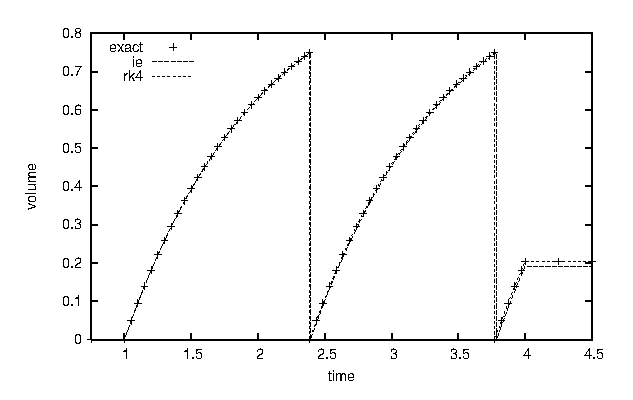
\epsfig{file=cont_models_figs/bucket.eps}
\caption{Volume of the bucket as a function of time when the spigot is opened at $t=1$ and closed at $t=4$.}
\label{fig:bucket}
\end{figure}
